\documentclass[journal]{IEEEtran}
\usepackage[utf8]{inputenc}
\usepackage{cite}
\usepackage[pdftex]{graphicx}
\usepackage{amsmath}
\usepackage{mathtools}
\usepackage{amsfonts}
\usepackage{amssymb}
\usepackage{bm}
\usepackage{hyperref}
%\usepackage{flushend}
\usepackage{balance}
\usepackage[caption=false,font=normalsize,labelfont=sf,textfont=sf]{subfig}
\DeclareMathOperator*{\argmax}{arg\,max}
\author{Chan~Tong~Kou,
Yves~Chan,
Andrew~Taeyeon~Kim,
and~Pranav~Garg%
\thanks{Submitted April 6, 2017.}
}
\title{RNA Structure Prediction Using Nussinov's Algorithm With Four Russians Speedup}
\begin{document}
\markboth{CPSC 445 - Algorithms in Bioinformatics}%
{RNA folding}
\maketitle
\begin{abstract}
We report on the implementation and testing of two algorithms used to predict secondary structure of an RNA sequence. The four Russians technique, used to speed up Nussinov's dynamic programming algorithm, provides an improvement in time complexity but adds several preparation steps. Using an efficient implementation of this ``Two-Vector" algorithm and the original method, we obtain structures for sequences of various sizes to see if the improvement in performance is evident for typical lengths. Our results indicate a two to five fold reduction in runtime for 500 - 5000 base sequences. The predicted structures, however, are very different from those known experimentally because the simple scoring model cannot capture all interactions between bases.
\end{abstract}
%predicts the secondary structure of an RNA sequence by maximising the number of non-crossing matchings between complementary base pairs. For a sequence of length $n$, it takes $\pmb{O(n^3)}$ steps

\section{Introduction}
\IEEEPARstart{R}{NA} molecules are crucial to some of the most fundamental life processes: gene regulation and protein synthesis. They are found in all domains of life including viruses, and many perform highly conserved functions. The secondary and tertiary structures of these molecules are central to their function, and often it is the folded structure that is conserved, not the actual sequence. Numerous methods have been developed to model and predict this folding process. Unlike proteins, where the native structure can be easily determined by methods such as X-ray crystallography and NMR, RNAs are much harder to work with. Not only are ribonucleases notoriously difficult to eliminate, the folded structures of RNA molecules are extremely sensitive to temperature and usually do not survive the processing phases of these experiments.

Fortunately, computational methods have become quite reliable in recent years. There are methods to predict RNA structures by sequence comparison with known structures. Others try to find \textit{de novo} the most favourable configuration by minimising free energy. An early algorithm for \textit{de novo} structure prediction was proposed by Nussinov and Jacobson \cite{Nussinov1980}. This works by maximizing the number of non-crossing base pairs in a single RNA strand. For a sequence of length $n$, it takes $O(n^3$) steps to deterministically find an optimal structure.  In 2010, this algorithm was further improved by Frid and Gusfield \cite{Frid2010} using the Four Russians technique where the solutions to all possible subproblems (upto a certain size) are precomputed and stored. This ``Two-Vector" algorithm is able to give the same solution as Nussinov but in $O(n^3/\log{n})$ time. Parallelized versions of these algorithms, published by Venkatachalam, Gusfield and Frid \cite{Venkatachalam2014}, have a further $n$-fold speed-up each.

A theoretical improvement in time complexity is relevant for large datasets but sometimes due to the presence of large constants hidden in the big $O$ notation, these algorithms actually take longer than simpler but ``worse" algorithms for actual input sizes. We test this effect on the Two-Vector and Nussinov algorithms using biological sequences of typical lengths. We also examine the resulting structures and compare them to the known structures.

\section{Algorithms}
\subsection{Nussinov's Algorithm}
Given an RNA sequence, this algorithm looks for a secondary structure which maximises the number of non-crossing complementary base pairs, \textit{i.e}, \texttt{G-C} and \texttt{A-U}. The assumption of non-complementary base pairs is defined as follows: if in a sequence positions $i$ and $i'$ are paired respectively with $j$ and $j'$, then either $i<j<i'<j'$ (sequential pairs) or $i<i'<j'<j$ (nested pairs) | see Figure \ref{crossingRNA}. The algorithm proceeds by dynamic programming, calculating scores for larger sub-sequences by adding new residues on either side of a smaller sub-sequence.

\begin{figure}[h]
\centering
\subfloat[Non-crossing pairs]{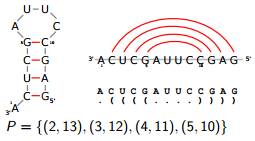
\includegraphics[width=2.5in]{fig1_1}%
%\label{fig_first_case}
}
\hfil
\subfloat[Pseudoknot]{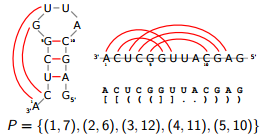
\includegraphics[width=2.5in]{fig1_2}%
%\label{fig_second_case}
}
\caption{Example of non-crossing base pairing vs. psudoknots. $P$ is the set of all pairs. Figure from \cite{MITfigure}}
\label{crossingRNA}
\end{figure}

Consider a two dimensional table $D$ where $D(i,j)$ denotes the maximum number of non-crossing base pairings for the subsequence from position $i$ to position $j$. After initialization, we only need to work only with the region $i<j$ of the table. Let length of the sequence be $n$.

%\begin{minipage}{0.9\columnwidth}
%\vspace{\baselineskip}
\subsubsection{Initialization}

For $-1 \leq j-i \leq M$:
\[
D(i,j)=0
\] where $M$ is the minimum gap between paired nucleotides to allow space for bending the backbone. Usually $M=4$.

\subsubsection{Recurrence}
We calculate the score for each $(i, j) : i<j\leq n$ by varying $i$ from $j-1$ to $0$ for each $j$:
\begin{equation}\label{recurrence}
D(i,j) = \max \begin{cases} b(S(i),S(j)) + D(i+1,j-1),\\
\max\limits_{i\leq k<j}[D(i,k) + D(k+1, j)]
\end{cases}
\end{equation}
where $b(S(i),S(j))$ is the score for pairing the residues at positions $i$ and $j$. It is $1$ if $S(i)$ is a complement of $S(j)$, and $0$ otherwise.

\subsubsection{ Termination and Traceback}

The best score is $D(1,n)$. During recurrence, we store how the best value was obtained in each step. This allows for traceback to reconstruct the pairings.

\subsubsection{Complexity}

    Out of the two terms in the recurrence expression \ref{recurrence}, the first term is calculated in constant time. The second term involves examining $O(n)$ values to find the maximum. Given there are $O(n^2)$ entries in the table, the total time complexity for this algorithm is $O(n^3)$.  
%\end{minipage}


\subsection{Two-Vector}

Dynamic programming algorithms typically proceed by filling out the answers to problems of increasing size in a table. The Four Russians Method is a tactic used to speed up calculations involved in filling up the table by pre-computing and storing answers to all possible pieces of the table. Imagine the table as being made up of blocks of some size. Each block is filled up using values stored in a boundary layer of cells, say top row and left column. If we can pre-compute what block values correspond to each set of boundary values we are able to speed up the table-filling process (provided we choose the block size appropriately).

This idea is ported over to our problem to speed up the calculation of the second term in the recurrence (\ref{recurrence}) by breaking the $i$\textsuperscript{th} row and $j$\textsuperscript{th} column into vectors of a particular length $q$. If we pre-computed the answer for each possible row vector with each possible column vector,  we could work vector by vector instead of cell by cell. This longer stride length gives a speed boost because we have far fewer terms to maximize over. To reduce the size of the lookup table, we work with difference vectors which store the difference between consecutive cells. This condenses many possible vectors into one entry in the table. Thus, we write the values of cells in a row vector of length $q$ starting at $(i,l)$ as
\[
\begin{array}{rl}

&D(i,l+p) = D(i,l) + V_p\text{, where }\\
&p\in \lbrace 0,...,q-1\rbrace\text{ and }V_p = \sum\limits_{i=0}^p v_i
\end{array}
\]
and $v$ is the horizontal difference vector in our lookup table. Entries in the horizontal difference vector are obtained as $D(i+i,j)-D(i,j)$ and an analogous vertical difference vector $\overline{v}$ is defined, whose values are $D(i,j+1)-D(i,j)$. The $v$ vectors are binary because entries in a row can only increase by either 1 or 0 caused by at most one new matched pair introduced in each step. The same works for $\overline{v}$ except that it contains either 0 or -1.

%To create a look-up table, we calculate and store the maximum score for each pair
\subsubsection{Pre-computation}
Let $v$ and $\overline{v}$ be written in a decimal representation by treating the vectors as numbers and dropping negative signs.

For each $(v,\overline{v})$, 
\[
T(v,\overline{v}) = \max\limits_{0\leq k\leq q}\left(\sum\limits_{i=0}^k v + \sum\limits_{j=0}^k \overline{v}\right)
\]

For traceback, we also store the $\argmax$.

\subsubsection{Initialization}
This is the same as before.

\subsubsection{Recurrence}

We calculate the score for each $(i, j) : i<j \leq n$ by varying $i$ from $j-1$ to $0$ for each $j$:

Let $(j-i) = g\times q +s$ where $s<q$. $g$ is number of blocks (``groups") and $s$ is number of cells that don't fit into blocks (``stragglers").

\begin{equation}\label{recurrence2}
D(i,j) = \max \begin{cases} b(S(i),S(j)) + D(i+1,j-1),\\
\max\limits_{i\leq k<s}[D(i,k) + D(k+1, j)],\\
%\max\limits_{i\leq k<g}[D(i,k) + D(k+1, j)],\\
\max\limits_{0\leq k<g} T\left( v(i,i+s+k\cdot q)\right.,\\ 
\hspace{20pt} \left.\overline{v}(i+1+s+k\cdot q, j) \right)


\end{cases}
\end{equation}
where $b(S(i),S(j))$ is the score for pairing the residues at positions $i$ and $j$. It is $1$ if $S(i)$ is a complement of $S(j)$, and $0$ otherwise.
\subsubsection{Termination and Traceback}
This is the same as before.

\subsubsection{Complexity}

In the pre-computation step, the first entry in each difference vector is set to zero so we omit those in the table. This gives us $O(2^{q-1})$ vectors to pre-compute, each taking $O(q)$ time. So pre-computing takes $O(q\times 2^{q-1})$ time In the recurrence step, we now step $q$ cells at a time, so the comparison is between $O(n/q)$ values. Since there are $O(n^2)$ cells, the recurrence takes $O(n^3/q)$ time.

The total complexity is $O(n^3/q) + O(q\times 2^{q-1})$. By differentiating with respect to $q$ to find the minimum for this expression, we get
\[
2^{q-1} \times (q^4 - q^3 + q^2)= {n^3}
\]
Keeping in mind that we are working with functional forms in $O$ notation and not exact functions, we can drop the polynomial on the left to get that $q \sim \log(n)$ for optimal complexity which is $O(n^3/\log n)$.
%\begin{figure}[!t]
%\centering
%\includegraphics[width=2.5in]{myfigure}
% where an .eps filename suffix will be assumed under latex, 
% and a .pdf suffix will be assumed for pdflatex; or what has been declared
% via \DeclareGraphicsExtensions.
%\caption{Simulation results for the network.}
%\label{fig_sim}
%\end{figure}

%\begin{figure*}[!t]
%\centering
%\subfloat[Case I]{\includegraphics[width=2.5in]{box}%
%\label{fig_first_case}}
%\hfil
%\subfloat[Case II]{\includegraphics[width=2.5in]{box}%
%\label{fig_second_case}}
%\caption{Simulation results for the network.}
%\label{fig_sim}
%\end{figure*}

%\begin{table}[!t]
%% increase table row spacing, adjust to taste
%\renewcommand{\arraystretch}{1.3}
% if using array.sty, it might be a good idea to tweak the value of
% \extrarowheight as needed to properly center the text within the cells
%\caption{An Example of a Table}
%\label{table_example}
%\centering
%% Some packages, such as MDW tools, offer better commands for making tables
%% than the plain LaTeX2e tabular which is used here.
%\begin{tabular}{|c||c|}
%\hline
%One & Two\\
%\hline
%Three & Four\\
%\hline
%\end{tabular}
%\end{table}

\section{Implementation and Testing}

We implemented the two algorithms using C and C++. The source code is available on \href{https://github.com/Pranav-Garg/RNAfolding/tree/master/code}{Github}\footnote{https://github.com/Pranav-Garg/RNAfolding/tree/master/code}. We included methods to compare runtimes, and to compare outputs of the two methods.

For testing, known RNA structures, as found in nature were obtained using the STRAND search page \cite{strand} in BPSEQ format. The sequences from these reference structures were input into our program. The resulting structures were visualized in VARNA \cite{varna}. In case of similar looking structures, simple file comparison could be used on the formatted outputs to look for differences.

We tested these algorithms on several sequences. The t-RNA sequences are of length $\sim$ 70 and so their structures could be easily compared by eye against those from the database. Eight different sequences of varying lengths from 486 to 4381 were used for run-time analysis.

\begin{figure}[t]
\centering
\subfloat[]{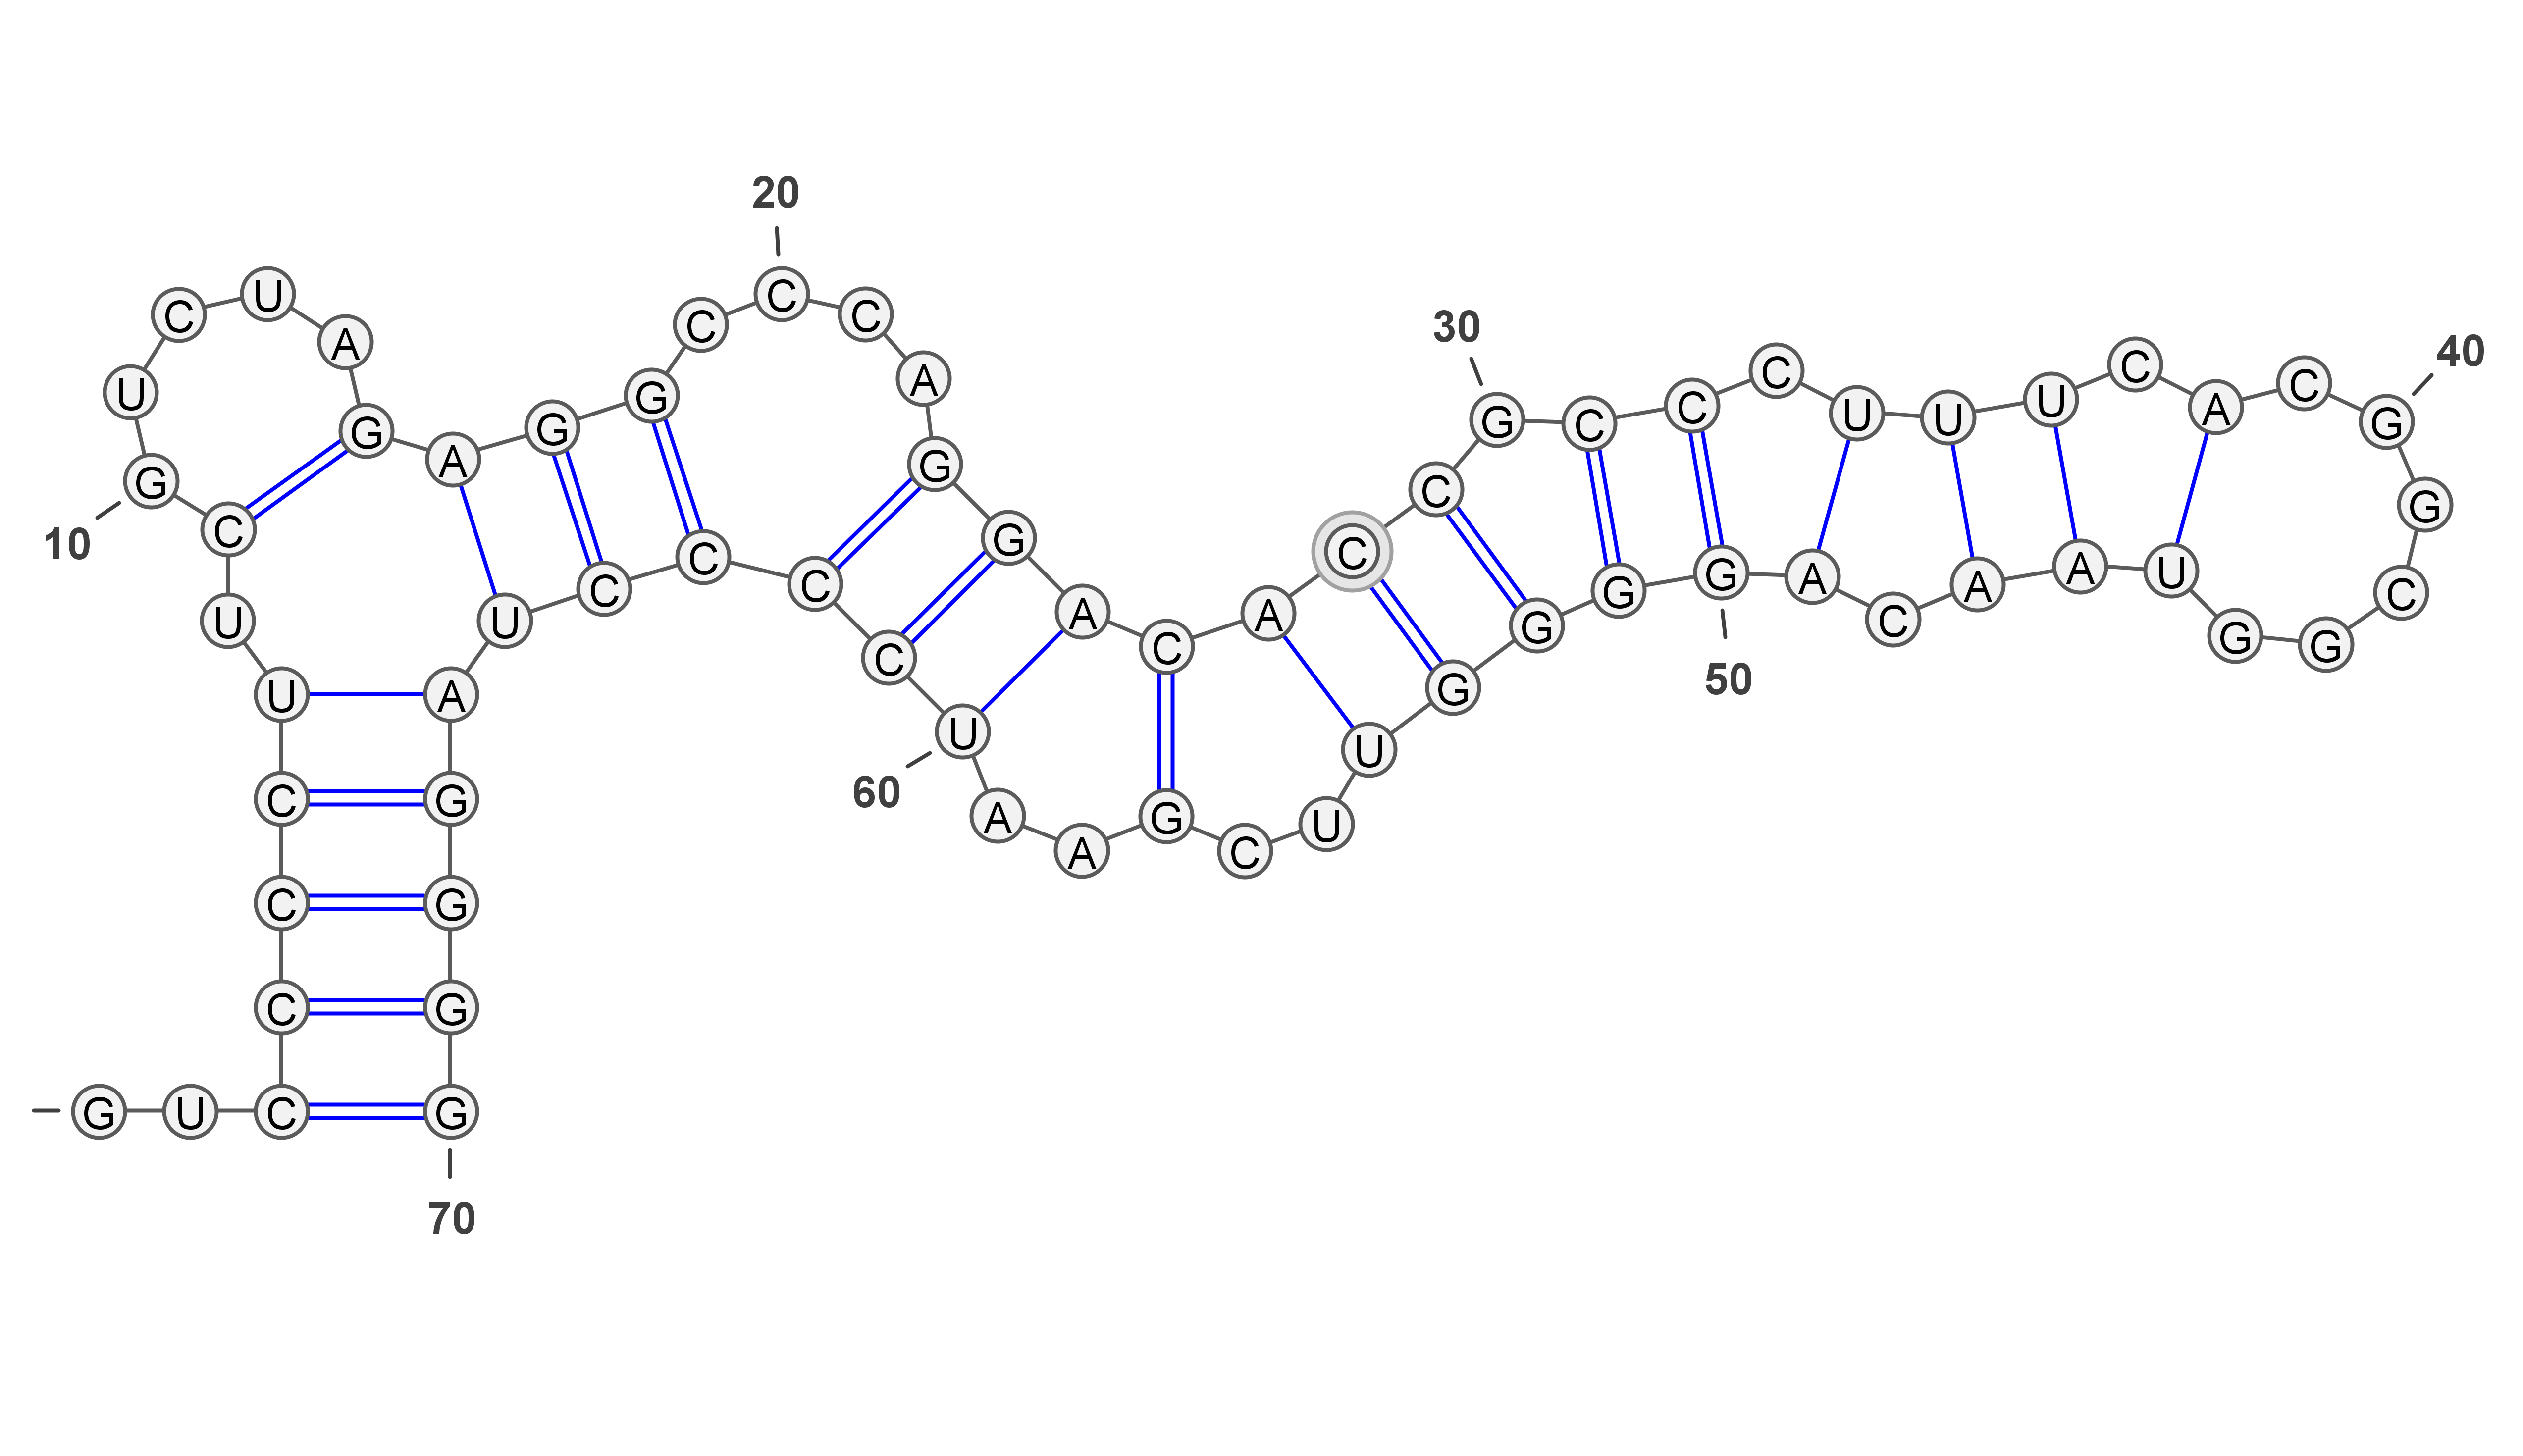
\includegraphics[width=2.5in]{fig2_1}%
%\label{fig_first_case}
}
\hfil
\subfloat[]{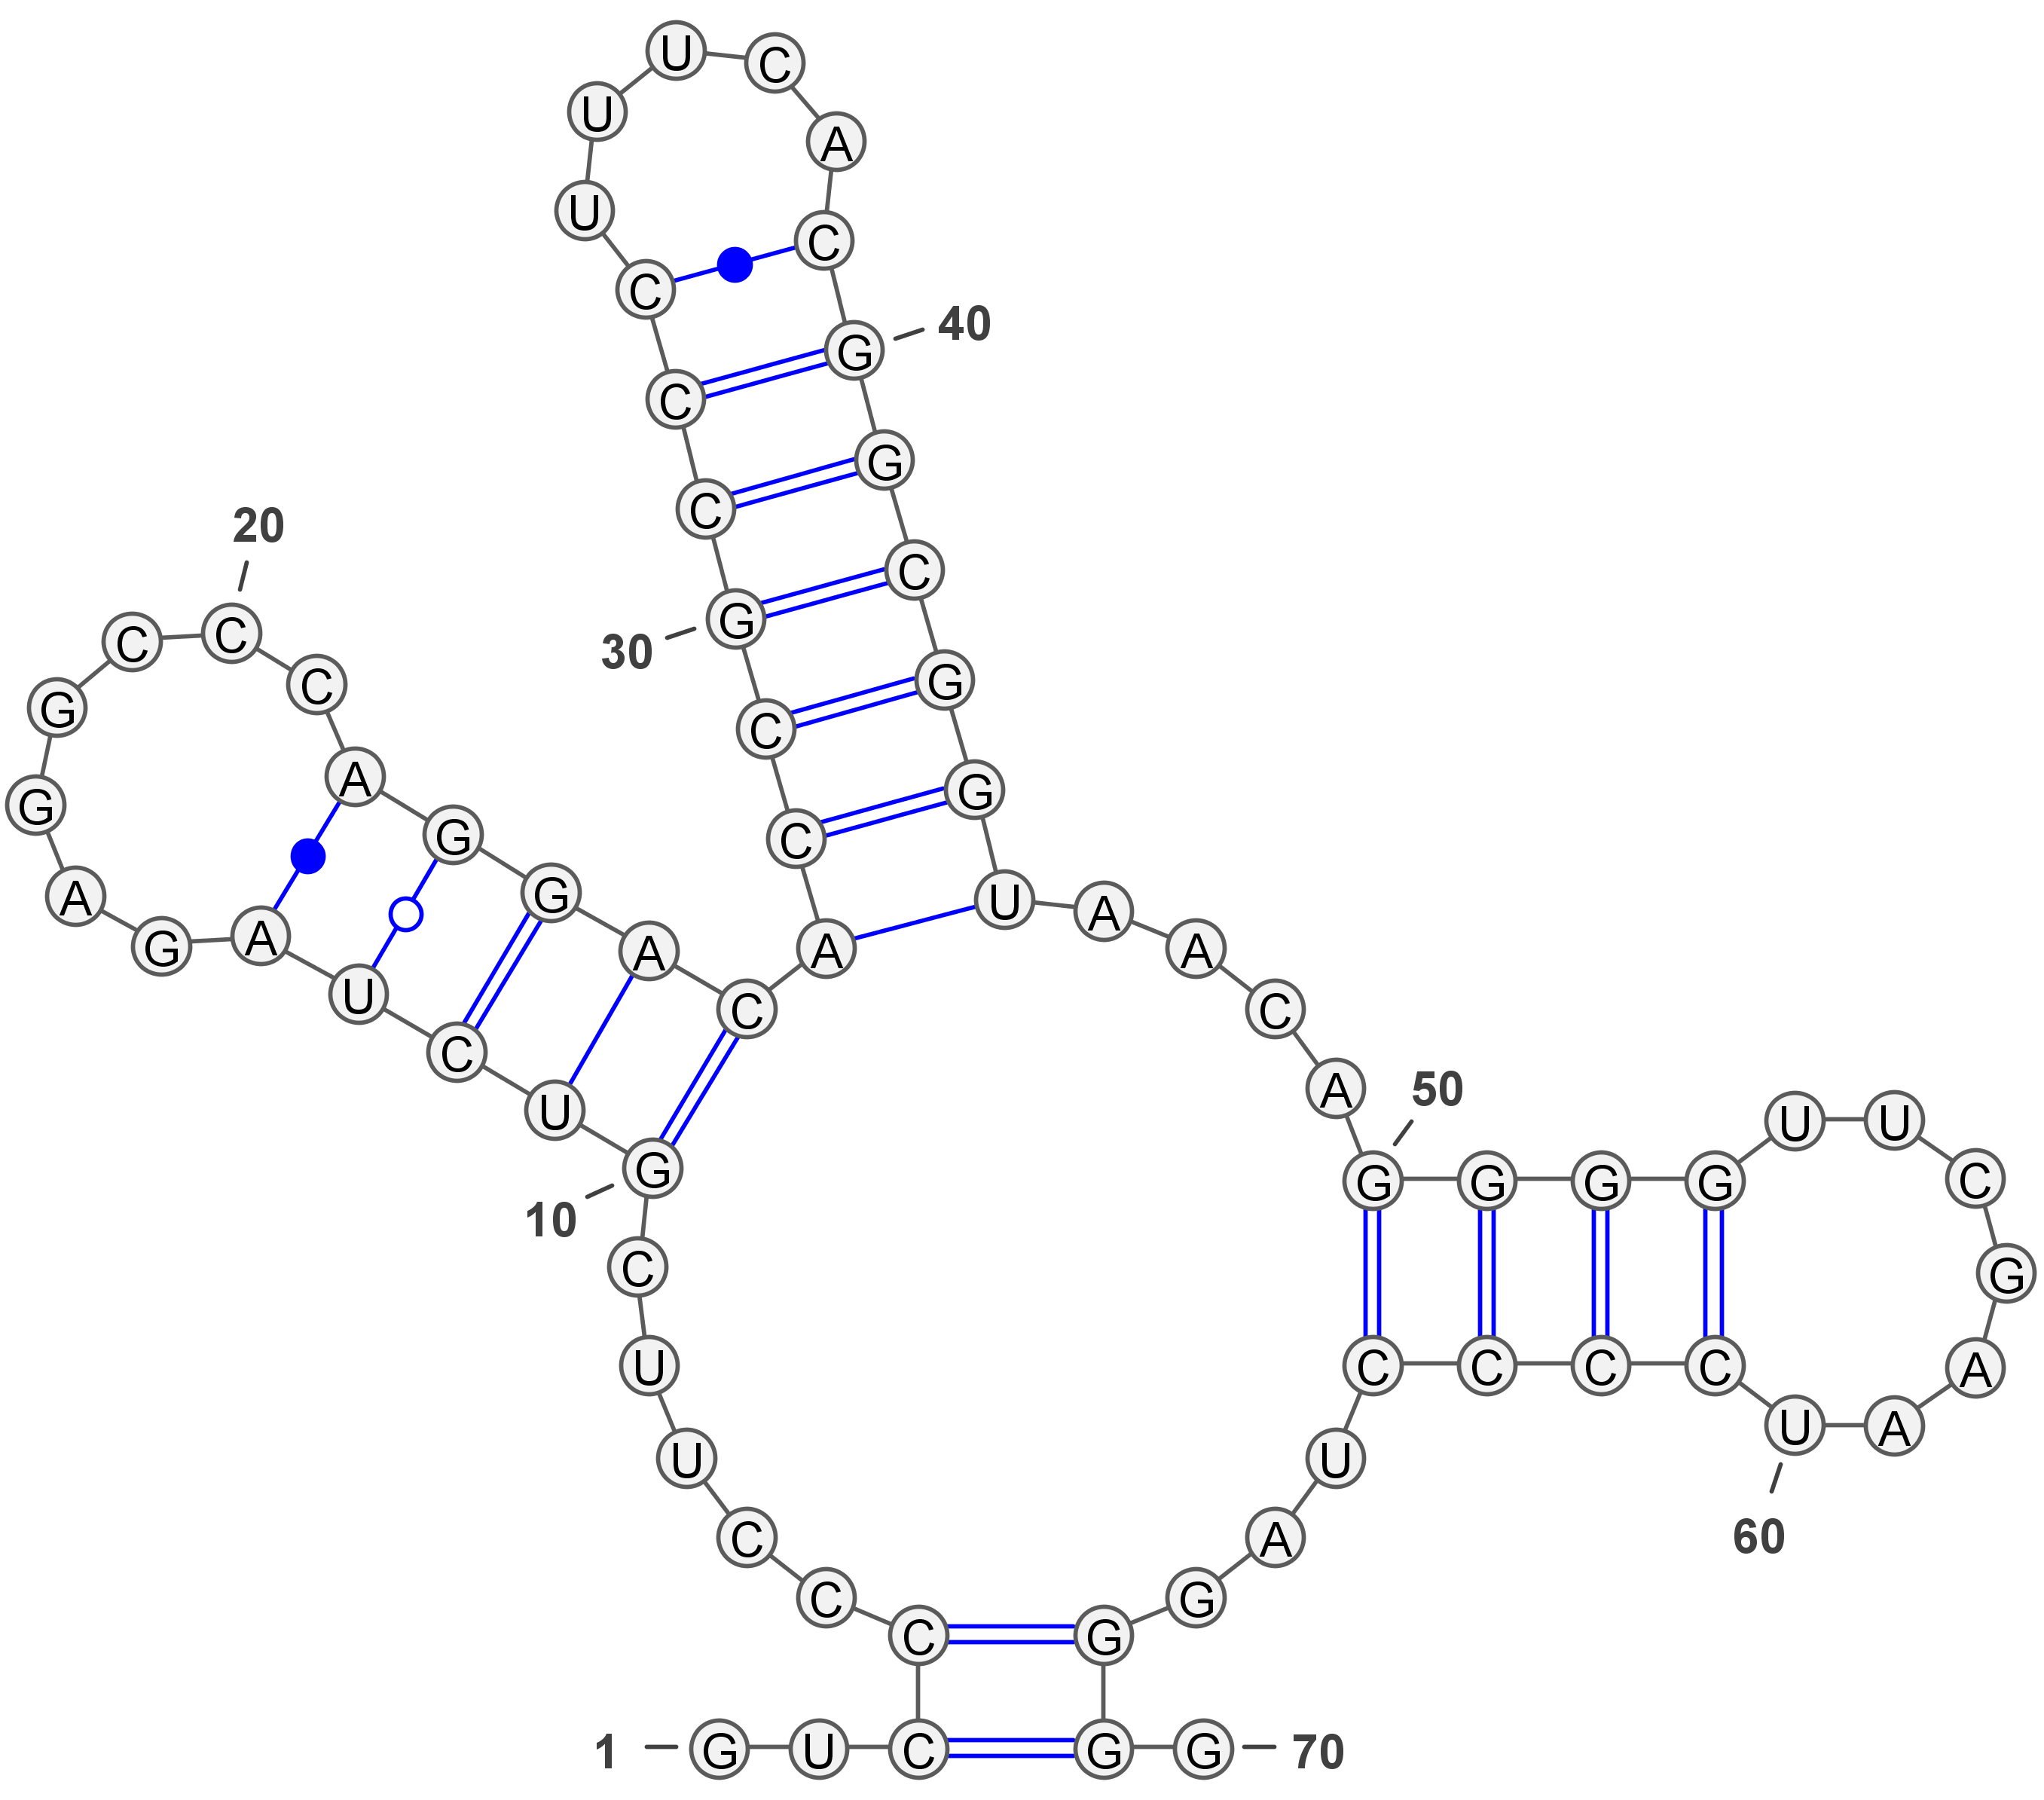
\includegraphics[width=2.5in]{fig2_2}%
%\label{fig_second_case}
}
\caption{Stuctures of Glu-tRNA from \textit{Escherichia coli} (PDB ID: \texttt{2DET}, RNA STRAND \texttt{PDB\textunderscore 00999}), as predicted by our folding algorithms (a) and known structure (b). Notice the presence of seven small bulge loops in the predicted structure, four of size 1 at residues 10, 33, 37 and 48, two of size 2 from 54 to 60 and one of size 3 near residue 20. No such motifs exist in the known structure.}
\label{structures}
\end{figure}


\section{Results}


The two methods implemented produce exactly the same dynamic programming tables and therefore identical results, as expected.



The structure obtained for a t-RNA sequence is shown in Figure \ref{structures}. It is clear that there are large disparities between the natural observed structure and the predicted structure. This is a general feature of the outputs generated | the algorithm allows for some unrealistic features in the structures. The predicted structure clearly has more paired residues, which shows that it is not a flaw in the implementation.

Looking closer, we see that the predicted structure has long stem loops with little room for the backbone to bend in going from one to the other. It also has unaligned nucleotides bulging outward from an aligned region. These bulge loops can actually be quite destabilizing for the structure in reality because they interrupt stacking of aromatic rings between adjacent residues. These features indicate that a better scoring model is needed to correctly penalise these features. The best way to account for such effects is to base the calculation on free energy contributions of each interaction between bases, as proposed by Zuker \cite{zuker}.

The runtime analysis is shown in Table \ref{table} and Figures \ref{runtime} and \ref{runtime_analysis}. The Two-Vector method outperforms the Nussinov algorithm in all cases. Runtime for short sequences was not available because it was too small to measure. The slopes in the log-log plots are close to 3 and clearly smaller for the Two-Vector algorithm which is consistent with our complexity analysis.




\section{Conclusion}
A variety of interactions contribute to the RNA secondary structure. The na\"{\i}ve scoring method used in Nussinov's algorithm is unable to take them all into account therefore giving structures that barely resemble those seen in nature. However, it was the first dynamic programming algorithm to address the problem of RNA secondary structure prediction. Many algorithms today follow the same computation schemes and therefore any strategy to speed up this algorithm can be applied to present day algorithms. We found that the Two-Vector method provides a two to five fold improvement in speed for sequences between 500 and 5000 bases long. This improvement could be valuable to Zuker's Algorithm which performs many floating point operations in every iteration.

\begin{table}[t]
%\renewcommand{\arraystretch}{1.3}
\caption{Runtime Data}
\label{table}
\centering
\begin{tabular}{|c|c|r|r|}
\hline
STRAND ID & Length & Nussinov (s) & Two-Vector (s)\\
\hline
ASE\textunderscore 00102 & 486 & 0.09375 & 0.06250\\
CRW\textunderscore 00432 & 950 & 0.73438 & 0.29688\\
CRW\textunderscore 00253 & 1522 & 3.42188 & 1.34375\\
CRW\textunderscore 00330 & 1995 & 9.46875 & 3.31250\\
CRW\textunderscore 00522 & 2700 & 27.48438 & 6.76562\\
PDB\textunderscore 00796 & 3009 & 41.37500 & 9.35938\\
CRW\textunderscore 00524 & 3539 & 72.21875 & 17.17188\\
CRW\textunderscore 00528 & 4381 & 147.85938 & 32.54688\\
\hline
\end{tabular}
\end{table}

\begin{figure}[t]
\centering
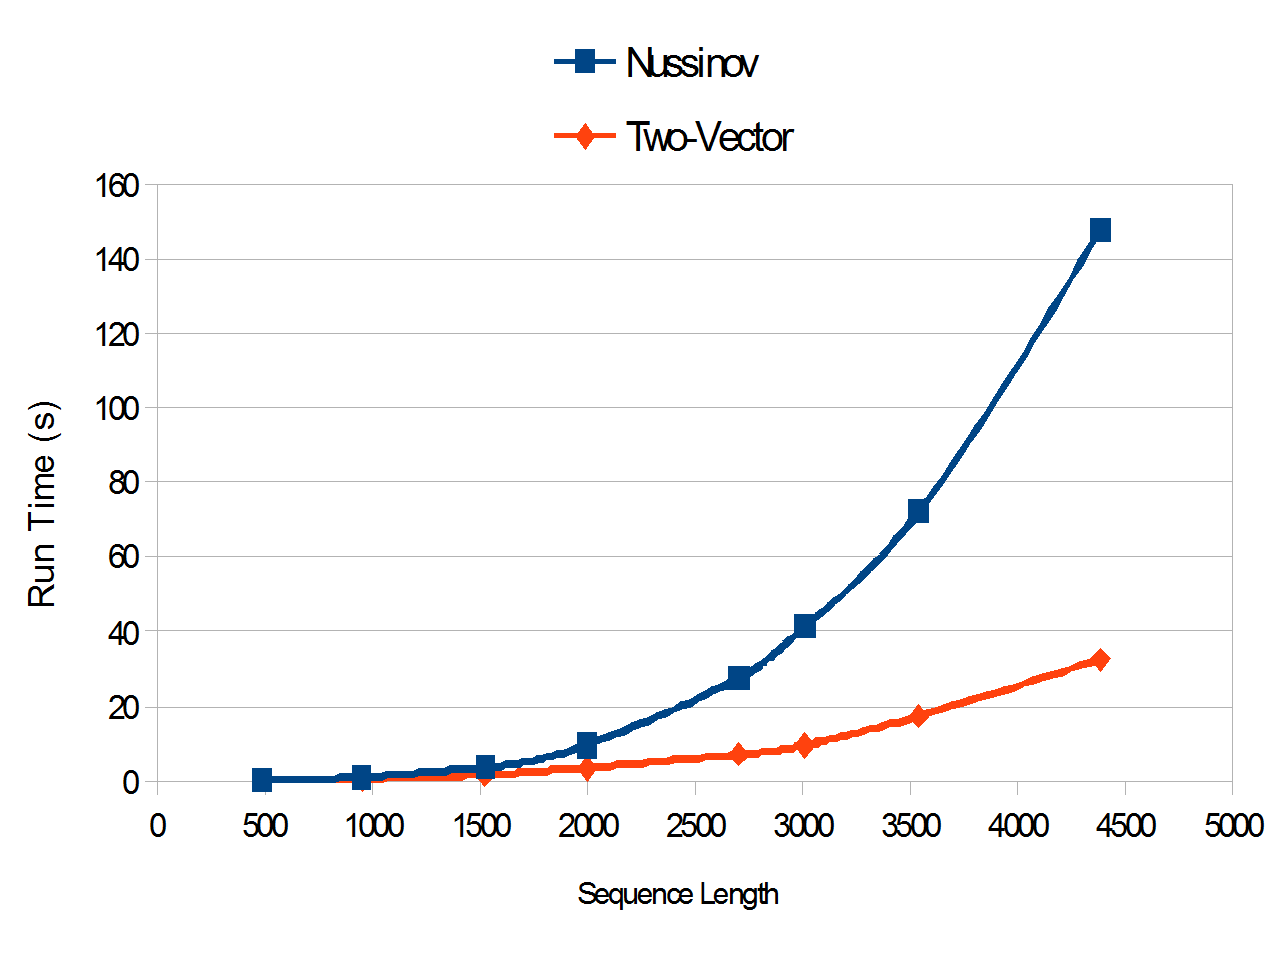
\includegraphics[width=3.0in]{fig3_1}%
%\label{fig_first_case}

\caption{Plot of runtime against sequence length.}
\label{runtime}
\end{figure}

\begin{figure*}[t]
\centering
\subfloat[]{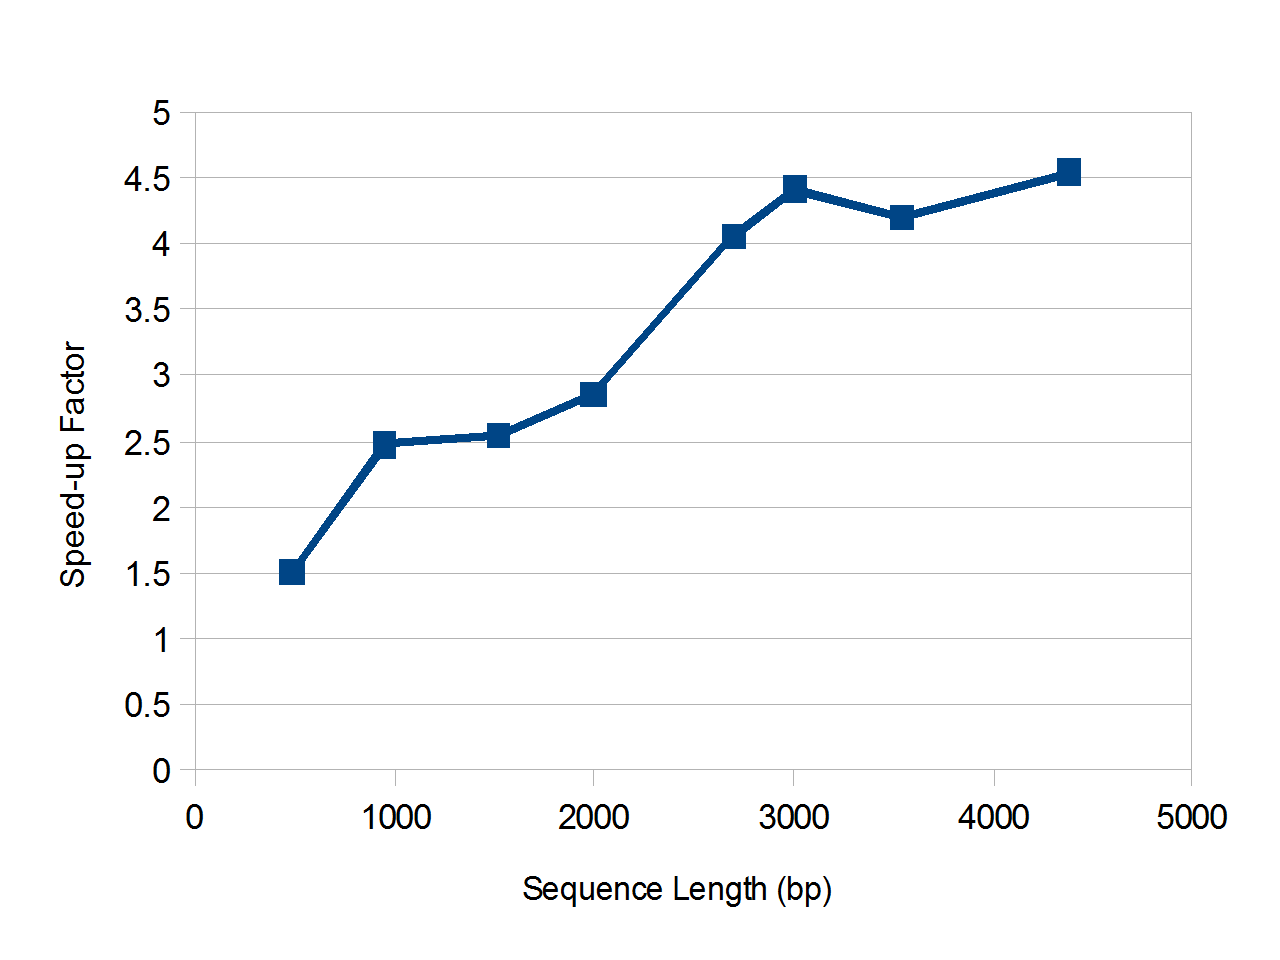
\includegraphics[width=3.0in]{fig3_2}%
%\label{fig_second_case}
}
\hfil
\subfloat[]{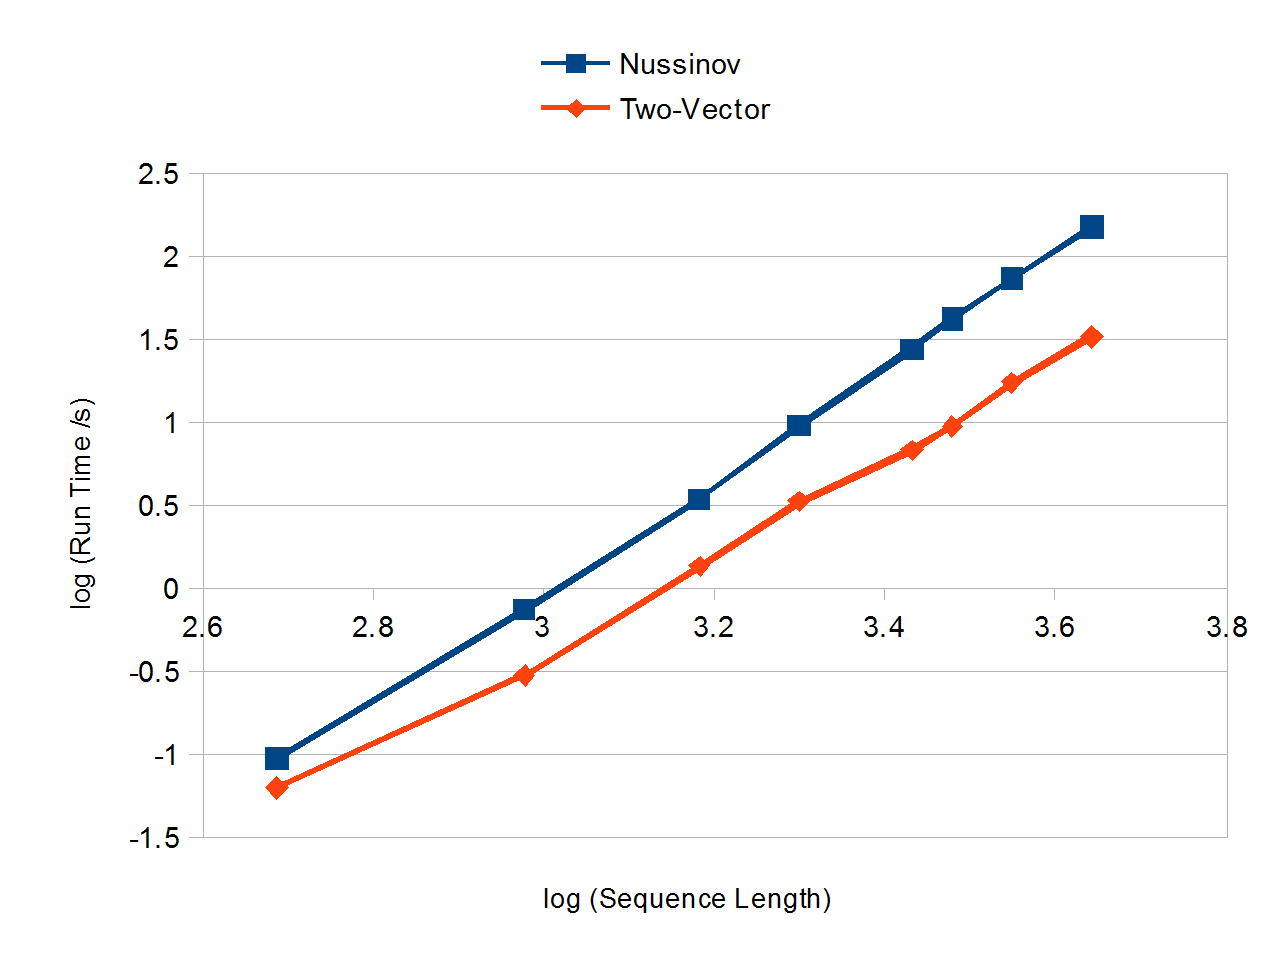
\includegraphics[width=3.0in]{fig3_3}%
%\label{fig_second_case}
}
\caption{Analysis of runtimes. The speed-up factor increases with length of sequence (a). The log-log plot is used to observe the scaling behaviour of runtime (b). Slopes of best-fit lines (not shown) are 3.387 and 2.875 for Nussinov and Two-Vector algorithms respectively. The runtime scales roughly as the cube of the sequence length the exponent is indeed lower for the Two-Vector method. }
\label{runtime_analysis}
\end{figure*}
%
%\appendices
%\section{Proof of the First Zonklar Equation}
%Appendix one text goes here.

% you can choose not to have a title for an appendix
% if you want by leaving the argument blank

%\section*{Acknowledgment}
%The authors would like to thank the instructor for our course Manuch Jan for ???


%\newpage
\balance
%\IEEEtriggeratref{8}
\bibliographystyle{IEEEtran}
% argument is your BibTeX string definitions and bibliography database(s)
\bibliography{RNAfold}

\end{document}

